% IITB CSE RISC Poster Template
% Credits: https://github.com/andiac/gemini-cam
% a fork of https://github.com/anishathalye/gemini
% also refer to https://github.com/k4rtik/uchicago-poster

\documentclass{beamer}

\usepackage[T1]{fontenc}
\usepackage{lmodern}
\usepackage[orientation=portrait,scale=1.0]{beamerposter}
\usepackage{graphicx}
\usepackage{booktabs}
\usepackage{tikz}
\usepackage{pgfplots}
\usepackage{anyfontsize}
\usepackage{blkarray}
\usepackage{listings}
\usepackage{tcolorbox}  % Import tcolorbox for rounded blocks
\usepackage{xcolor}  % Ensure xcolor package is included

\geometry{papersize={36in,48in}}
\usetheme{gemini}
\pgfplotsset{compat=1.14}
\usecolortheme{nott}

%\lstset{numbers=left, numberstyle=\tiny, stepnumber=1,firstnumber=1,
%  numbersep=5pt,language=Java,
%  stringstyle=\ttfamily,
%  basicstyle=\footnotesize,
%  showstringspaces=false
%}

\definecolor{customblue}{RGB}{187,218,233}  % Define #8AC9E1 as customblue
\setbeamercolor{block body}{fg=black, bg=rgb, bg=customblue!50!white}   % Body background color
%\setbeamertemplate{blocks}[rounded][shadow=false]

% If you have N columns, choose \sepwidth and \colwidth such that
% (N+1)*\sepwidth + N*\colwidth = \paperwidth
\newlength{\sepwidth}
\newlength{\colwidth}
\setlength{\sepwidth}{0.00\paperwidth}
\setlength{\colwidth}{0.45\paperwidth}
\lstset{
  language=Java,
  numbers=right,
  showstringspaces=false
  stringstyle=\ttfamily,
  basicstyle=\fontsize{26pt}\selectfont\ttfamily,  % Set font size to 14pt
  captionpos=b,
  backgroundcolor=\color{customblue!10!white},   % Background color
  numberstyle=\color{red!50!white},            % Line number color
  keywordstyle=\color{blue}\bfseries,  % Keywords color
  commentstyle=\color{green!50!black}, % Comment color
  stringstyle=\color{red!50!black}              % String color
}

% Define a new custom rounded block style with padding
\newtcolorbox{roundedbeamerblock}[2][]{%
  colback=customblue!20,  % Light blue background
  colframe=customblue,    % Border color
  coltitle=black,         % Title text color
  fonttitle=\bfseries,    % Bold title
  colbacktitle=customblue!60, % Title background color
%  sharp corners=south,    % Keeps top corners sharp (like Beamer)
  arc=15pt,               % Adjust roundness (Increase for more rounded effect)
  boxrule=1pt,            % Border thickness
  title={#2},             % Title argument
  #1,                     % Additional user options
  left=6mm,               % Left padding
  right=18mm,              % Right padding
  top=5mm,                % Top padding
  bottom=3mm              % Bottom padding
}

% Define a new custom rounded block style with padding
\newtcolorbox{roundedalertblock}[2][]{%
  colback=red!10,  % Light blue background
  colframe=red!40,    % Border color
  coltitle=black,         % Title text color
  fonttitle=\bfseries,    % Bold title
  colbacktitle=red!20, % Title background color
%  sharp corners=south,    % Keeps top corners sharp (like Beamer)
  arc=15pt,               % Adjust roundness (Increase for more rounded effect)
  boxrule=1pt,            % Border thickness
  title={#2},             % Title argument
  #1,                     % Additional user options
  left=6mm,               % Left padding
  right=18mm,              % Right padding
  top=5mm,                % Top padding
  bottom=3mm              % Bottom padding
}


% Define a new custom rounded block style with padding
\newtcolorbox{roundedexampleblock}[2][]{%
  colback=green!10,  % Light blue background
  colframe=green!40,    % Border color
  coltitle=black,         % Title text color
  fonttitle=\bfseries,    % Bold title
  colbacktitle=green!20, % Title background color
%  sharp corners=south,    % Keeps top corners sharp (like Beamer)
  arc=15pt,               % Adjust roundness (Increase for more rounded effect)
  boxrule=1pt,            % Border thickness
  title={#2},             % Title argument
  #1,                     % Additional user options
  left=6mm,               % Left padding
  right=18mm,              % Right padding
  top=5mm,                % Top padding
  bottom=3mm              % Bottom padding
}
\renewcommand{\normalsize}{\fontsize{35pt}{10pt}\selectfont}

\newcommand{\separatorcolumn}{\begin{column}{\sepwidth}\end{column}}

\title{POLYGLOT PROGRAM OPTIMIZATION}

\author{Anadi Mitra \hspace{3mm} and \hspace{3mm} Prof. Manas Thakur}

%\institute[shortinst]{\inst{1} CSE IITB \samelineand \inst{2} CSE IITB}

\footercontent{
  \href{https://www.cse.iitb.ac.in/plato/}{
\includegraphics[height=1.7cm]{images/plato} www.cse.iitb.ac.in/plato} \hfill
PLACID 2025
}

\logoleft{\hspace{20ex}
\includegraphics[height=6.5cm]{assets/logos/iitb-white.png}}
\logoright{
\includegraphics[height=5.5cm]{assets/logos/cse-dept-logo.png}}

% ====================
% Body
% ====================

\begin{document}

% Refer to https://github.com/k4rtik/uchicago-poster
% logo: https://www.cam.ac.uk/brand-resources/about-the-logo/logo-downloads
% \addtobeamertemplate{headline}{}
% {
%     \begin{tikzpicture}[remember picture,overlay]
%       \node [anchor=north west, inner sep=3cm] at ([xshift=-2.5cm,yshift=1.75cm]current page.north west)
%       {\includegraphics[height=7cm]{logos/unott-logo.eps}}; 
%     \end{tikzpicture}
% }

\begin{frame}[t]
\begin{columns}[t]
\separatorcolumn
\begin{column}{\colwidth}
  \vspace{50mm}
  \begin{roundedbeamerblock}{1. What Is Polyglot Programming}
    \baselineskip 50pt
    \vspace{5mm}
    \begin{itemize}
        \item Writing software using multiple programming languages within a single program.
    \vspace{4mm}
        \item These program runs within a common execution environment.
    \vspace{5mm}
    \end{itemize}

\end{roundedbeamerblock}

  \vspace{40mm}
  \begin{roundedexampleblock}{Example 1: Java-Python Polyglot Program}
\lstinputlisting{code/PolyglotExample.java}
\end{roundedexampleblock}

  \vspace{40mm}
  
\begin{roundedbeamerblock}{2. Be A Polyglot Programmer}
    \vspace{5mm}
    \begin{itemize}
        \item Allows you to leverage the strengths of different languages for specific tasks.
    \vspace{5mm}
        \item Enhances flexibility and improve performance.
    \vspace{5mm}
        \item Use existing libraries, increases development speed.
    \vspace{6mm}
        \end{itemize}
    \textbf{Use case}: Python for simplicity, Java for performance, and JavaScript for web integration.

\end{roundedbeamerblock}

  \vspace{50mm}
  \begin{roundedbeamerblock}{3. Run Polyglot Programs}


    \vspace{5mm}
    Quite a few polyglot runtimes available:
    \vspace{2mm}
    \begin{itemize}
        \item GraalVM
        \vspace{5mm}
        \item Jupyter Notebooks
        \vspace{5mm}
        \item .NET CLR
        \vspace{5mm}
        \item Node.js with WebAssembly
    \end{itemize}

\end{roundedbeamerblock}

  \vspace{50mm}
  \begin{roundedbeamerblock}{4. GraalVM Architecture}

    \vspace{5mm}
    \begin{itemize}
        \item A high-performance runtime that allows you to run polyglot programs.
        \vspace{5mm}
        \item Uses JIT compiler to optimize JVM programs.
    \end{itemize}
    \begin{figure}[h]
        \centering
        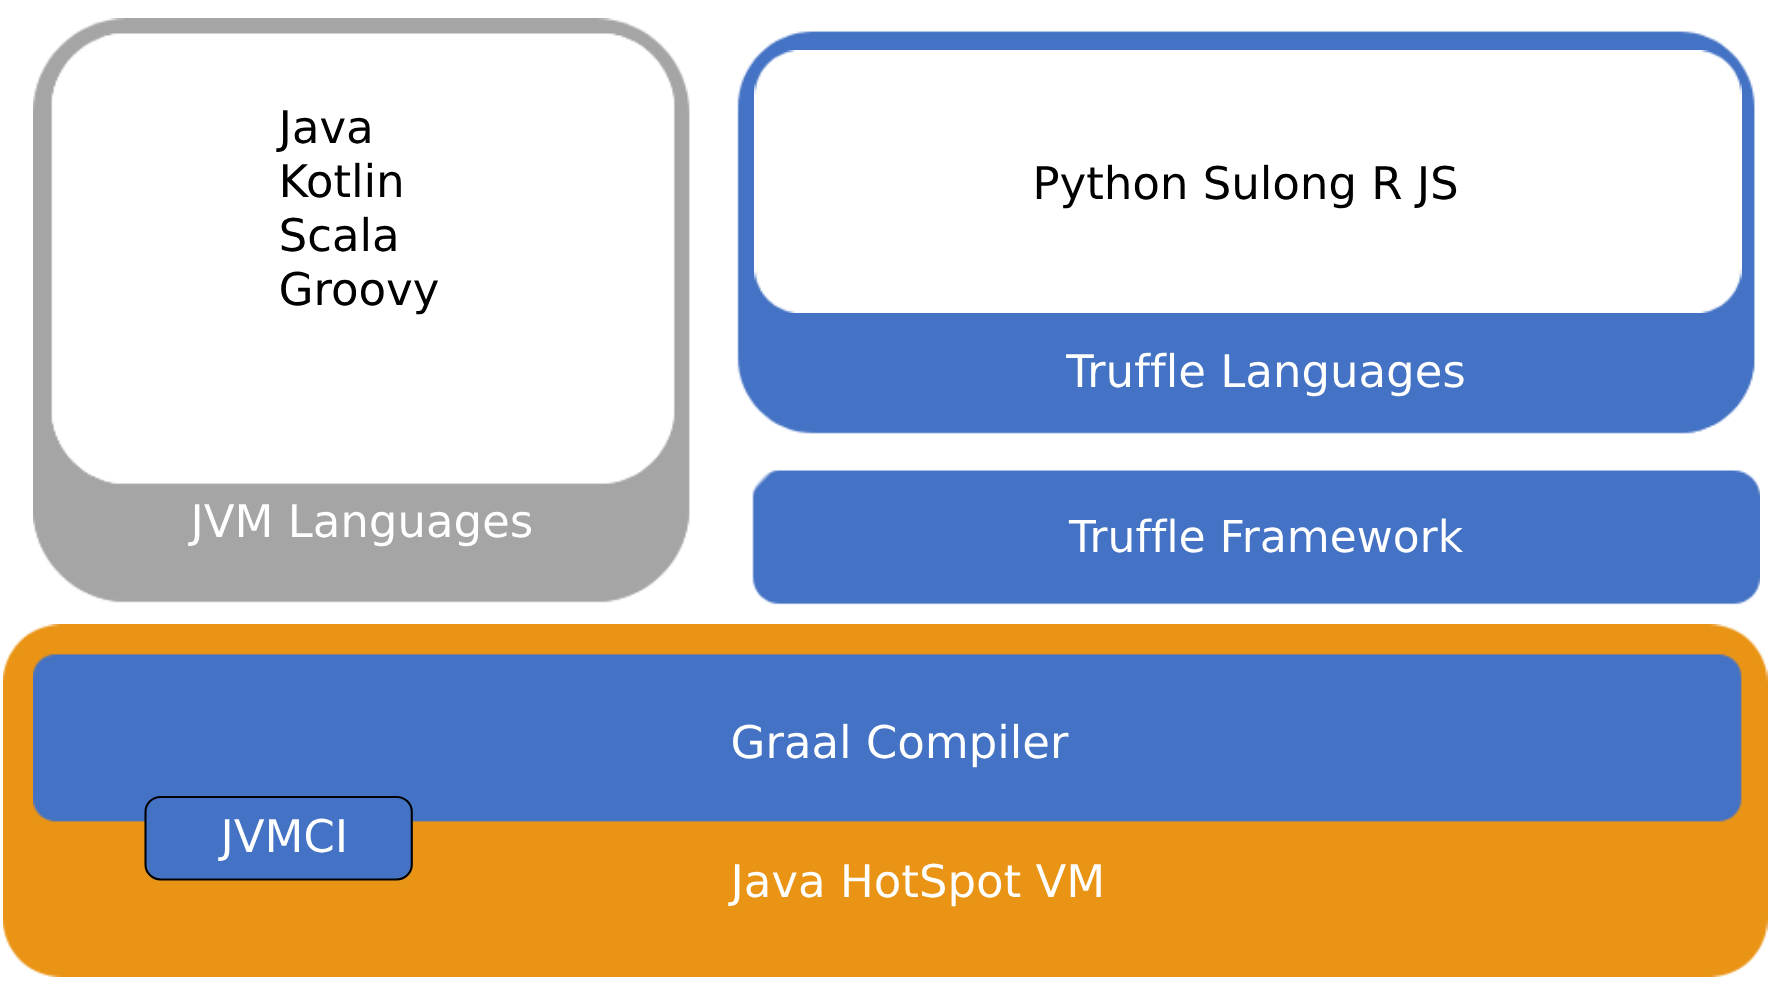
\includegraphics[width=0.9\textwidth]{images/graalvmArchitecture}
        \caption{GraalVM}
        \label{fig:graalvmArchitecture}
    \end{figure}

\end{roundedbeamerblock}

  \vspace{50mm}
\end{column}
%%%%%%%%%%%%%%%%%%%%%%%%%%%%%%%%%%%%%%%%%%%%%%
\separatorcolumn
\begin{column}{\colwidth}

  \vspace{50mm}
  \begin{roundedexampleblock}{Example 2: Escape Analysis}
\lstinputlisting{code/Escape.java}
\end{roundedexampleblock}

  \vspace{50mm}
  \begin{roundedbeamerblock}{5. Problem With Polyglot Programs}

    \vspace{7mm}
    \begin{itemize}
        \item \textbf{Polyglot runtimes} are complex, though abstracts language boundaries.
        \vspace{8mm}
        \item \textbf{Debugging \& Readability} of such programs can be challenging.
        \vspace{8mm}
        \item \textbf{Traditional analysis} tools does not fully support polyglot code analysis.
    \end{itemize}

\end{roundedbeamerblock}
  \vspace{50mm}
  \begin{roundedalertblock}{Challenge}
    \vspace{5mm}
    \baselineskip 50pt

    \begin{itemize}
        \item \textbf{Inter-Language Program Analyses}\par
            Language boundaries in polyglot programs limit the analyses, making optimization challenging.
        \item \textbf{JIT Compilation And Dynamic Languages}\par
        JIT makes program analysis harder due to runtime dynamism and partially available programs.\par
    \end{itemize}

\end{roundedalertblock}

  \vspace{40mm}
  \begin{roundedbeamerblock}{6. Key Idea: A Hybrid Approach}
    \vspace{5mm}
    Dependencies are generated \textbf{statically} for analysis.\par
    \vspace{5mm}
    Resolve them \textbf{dynamically} when whole program is available.\par
    \vspace{5mm}
%    For \par

\end{roundedbeamerblock}

  \vspace{50mm}
  \begin{roundedbeamerblock}{7. Common Interface For Framework}
    \begin{figure}[h]
        \centering
        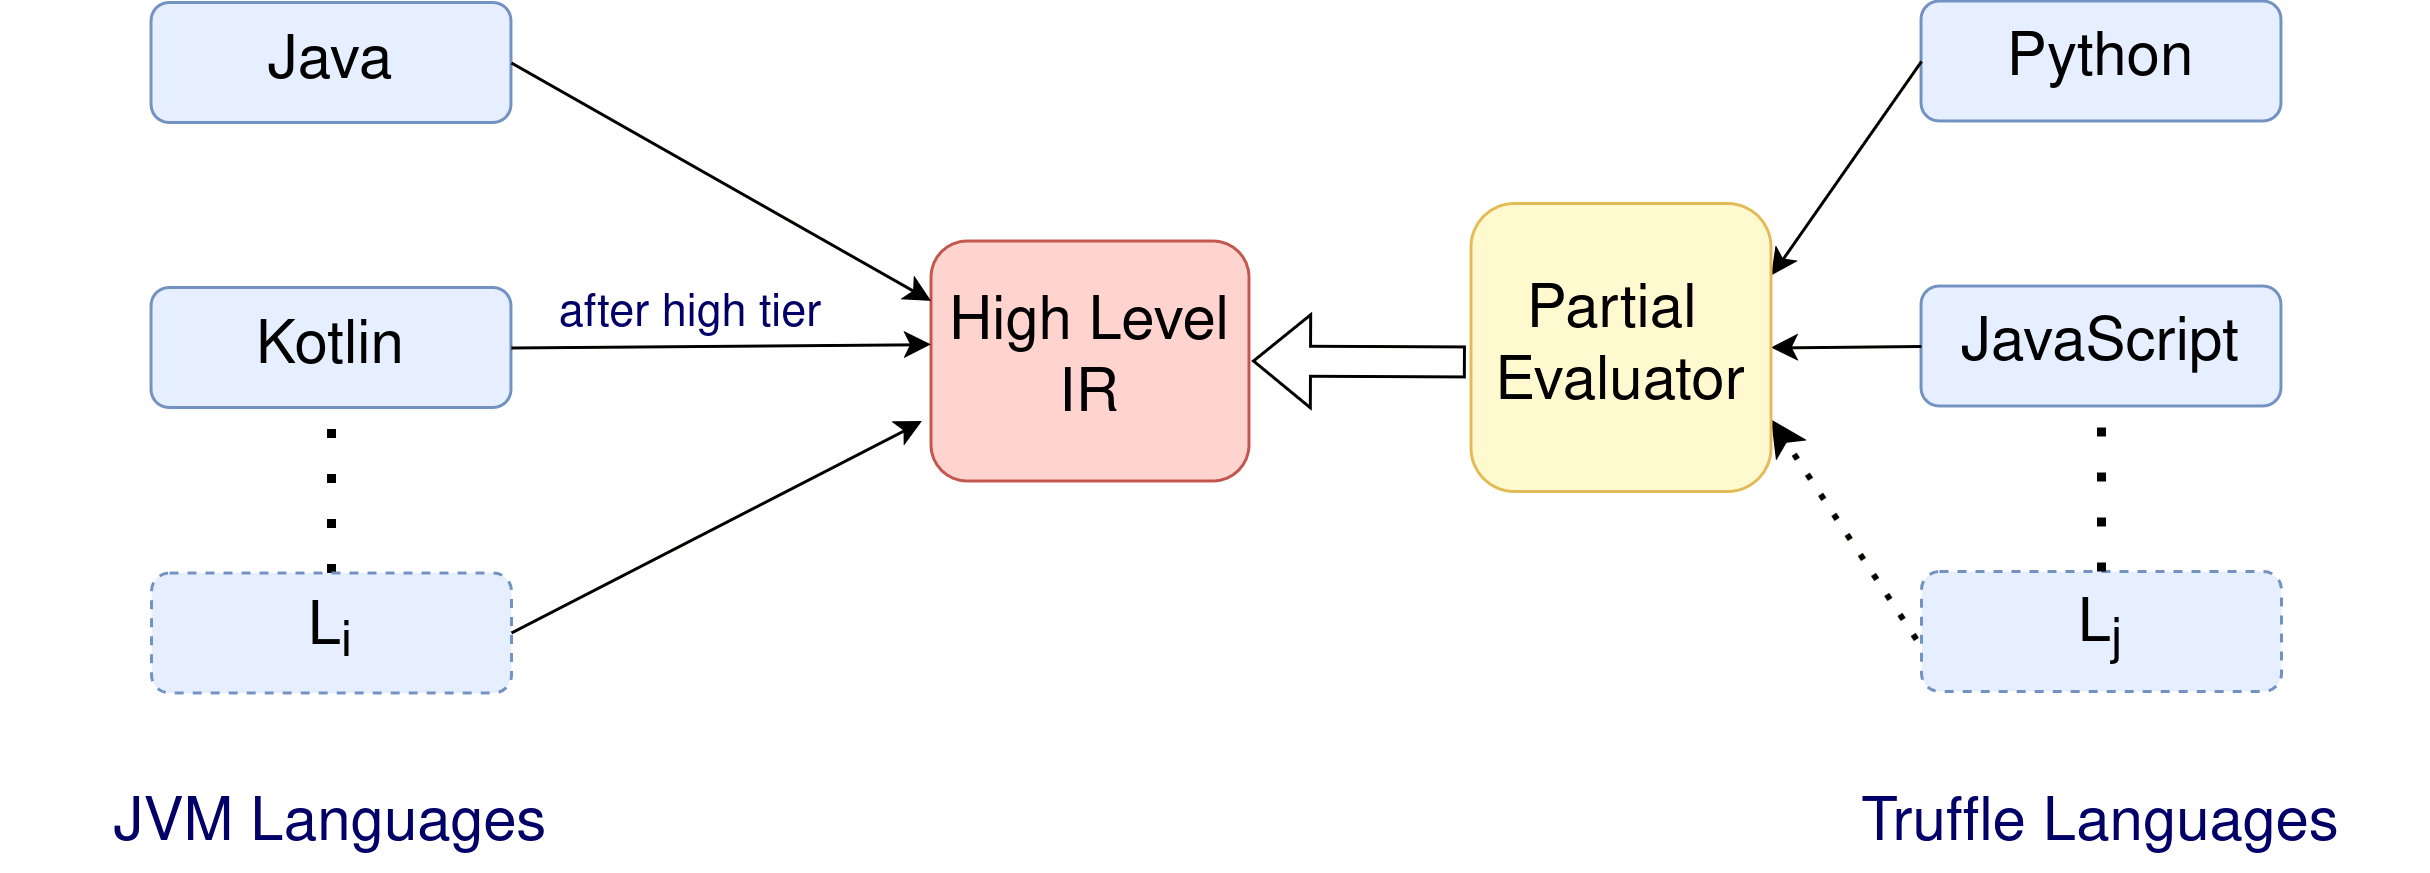
\includegraphics[width=1.0\textwidth]{images/common_interface}
        \caption{N\times M polyglot systems with a common interface}\label{fig:figure2}
    \end{figure}
\end{roundedbeamerblock}

%  \vspace{50mm}
%  \input{texBlocks/08-StaticallyMakeDependenciesAndResolveDynamically}
%  \vspace{50mm}
%  \begin{roundedbeamerblock}{JIT Compilation And Dynamic Languages}
    \vspace{5mm}
    JIT makes program analysis harder due to runtime dynamism and partially available programs.\par
    \vspace{5mm}
    Language boundaries also limit the analyses scope, making optimization more challenging.\par
    \vspace{5mm}

\end{roundedbeamerblock}


  \vspace{30mm}
  \begin{roundedbeamerblock}{References}
    \nocite{*}
    \footnotesize{\bibliographystyle{plain}\bibliography{poster}}
\end{roundedbeamerblock}



%  \begin{roundedbeamerblock}{References}
    \nocite{*}
    \footnotesize{\bibliographystyle{plain}\bibliography{poster}}
\end{roundedbeamerblock}

\end{column}
\end{columns}

\end{frame}

\end{document}
